\section{Discussion}
\label{sec:discussion}
The process of getting our results provided insight into the redundancies that exist within mobile web pages. We first observed that pages that are designed for mobile browsers are only a fraction of the size of pages designed for desktop browsers. In addition to size, we also know that the way that mobile sites are structured are inherently different through observation. Because of this, we decided that it was worth exploring the types of redundancies that exist within mobile sites. This information can be used in the future to examine how these redundancies are similar to or different from desktop browser site redundancies. It can also be used to design caches that will take advantage of the redundancy patterns that we find.  \\

At this point, we ran several experiments to find optimal chunk size. From our data, we found that a chunk size close to 10 bytes was optimal in the trade-off between obtaining a low miss-rate and reducing the number of bytes of fingerprints transferred back and forth between the proxy and mobile device. From the feedback we received after our presentation, we decided to implement the sliding window chunking methodology so that we wouldn't be constrained to a fixed chunk size and so that we would find a larger percent of deduplicated data. \\

Lastly, we simulated patterns of mobile web browsing to obtain an approximate result of how much we can expect to reduce bandwidth. We found that if the cache contains an older version of the page, and data from several similar pages, then (with a chunk size of 10 bytes) only about 20\% of the content is new and needs to be retreived from the proxy. \\

There were multiple design decisions that we considered before constructing the protocol. We designed our protocol such that fingerprint computation only occurs at the proxy. This is because mobile devices tend to have limited computational capacity and if the heavy lifting is deferred to the proxy, then the mobile device simply has to do look-ups to determine cache hits and misses. This means that we incur the overhead of passing fingerprints back and forth on the network, leading to possible latency, additional power consumption. In addition, it also reduces the benefits of bandwidth reductions obtained by chunking. We recognized there is an inefficiency that comes from the additional communication that needs to occur between the device and proxy of sending fingerprints. In addition, we recognized that using MRU eviction algorithm for our tests could have possibly restricted our bandwidth reduction. We implemented a modified version of the protocol to address these drawbacks, as proof of concept and for testing purposes, that is shown in figures. \\

\begin{figure}[h] 
\centering 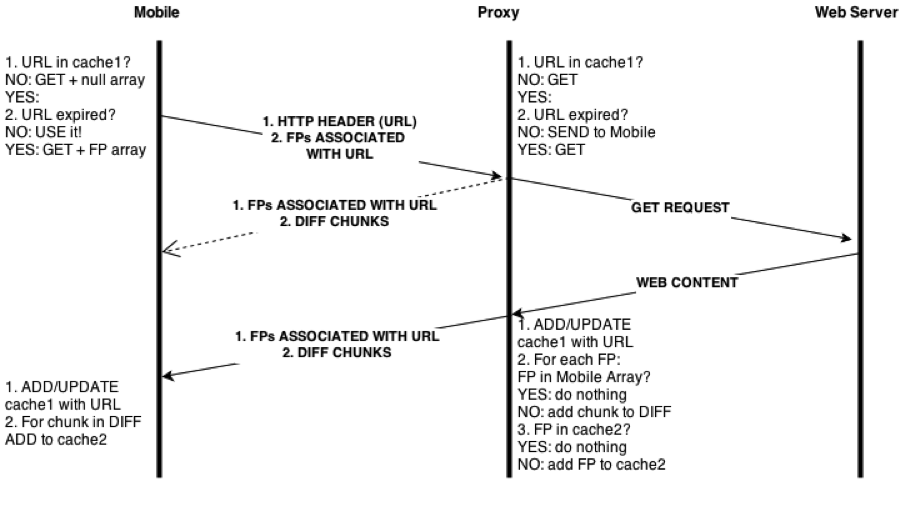
\includegraphics[scale=0.40]{images/urlcache-protocol.png}
\caption{Protocol. }
\end{figure} 

\begin{figure}[h] 
\centering 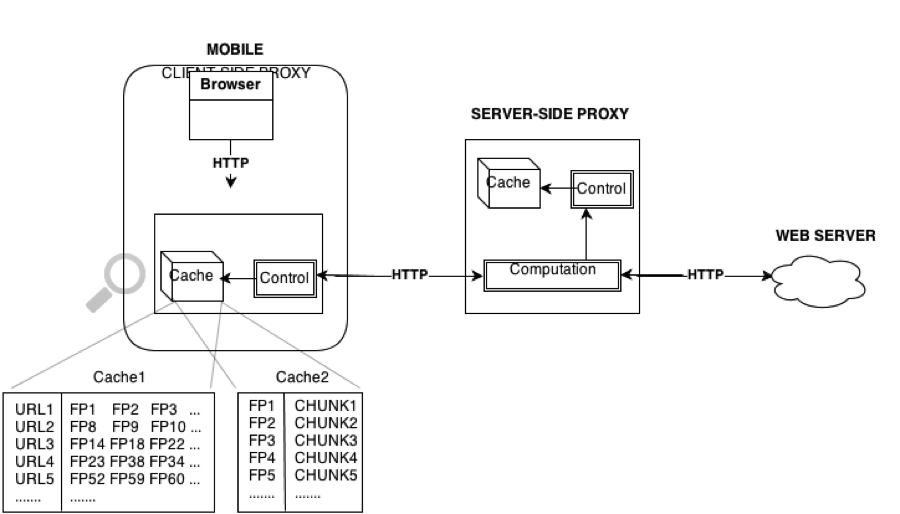
\includegraphics[scale=0.40]{images/url-cache-hl.png}
\caption{Url-Cache. }
\end{figure} 

The modified implementation works in the following way. In addition to the previous implementation, we added a url-cache, which maps each url request to the set of fingerprints that represent it. If the mobile device contains an older version, it sends the FP to the proxy along with the requested url. The proxy then sends back the diff between the mobile's fingerprints and fingerprints of fresh content which it either obtains from its own cache or from the web server. \\

The figure shows that it may be possible to reduce latency with this approach due to the decreased amount of communication that needs to occur between the proxy. In addition, preliminary testing during implementation showed that in some cases (dependent on the size of the page, and whether or not an older version of it was in the cache, and pattern of 'browsing') bandwidth. The fingerprint overhead remains on the same order because the fingerprint of the entire page still needs to be sent. The bandwidth reduction comes from a lower missrate afforded by the url cache.  \\

Some design things we are aware of but have not addressed are the following. We assume that each time we made a request that the content in our cache was not fresh, and we did not implement checking for freshness. We also attempted to collect data from various other websites but ran into several issues. Some websites don't have a different version for mobile devices at all. Some others had a different version, but did not use it as its response based on the User-Agent, and instead required a request of the mobile url. Redirects were also not handled in the way we obtained offline data. Furthermore, we did not check to see if the data was "cacheable" and assumed that all the websites we were working with had cacbeable content. Lastly, the results of our tests did not incorporate checks for content overlap between different chunks -  we now have a sliding window for chunking in place which is passed along the content stream to catch redundancies between different chunks that would not have been caught with fixed-sized chunks. \\

A last, but minor point is the consideration of how integrity of data is affected by possible collision due to fingerprinting. We assume that we do not get collision because the size of our content is small enough that the risk of collision is negligible. 

Some assumptions

%
%Weaknesses

%Assumptions
%- mobile calculating fingerprints
%- expiration
%- cache - use of hashtable accurate?
%- cache size


%future: desktop vs mobile

%Experiments
%1. chunking vs non chunking
%2. webpage vs no webpage
%3. different types of caches
%4. Different chunk sizes
%5. fps misrate vs chunk/byte missrate
%6. Bytes transferred
%7. multiple mobiles
%8. collected data
%9. different cache types
%10. different chunk sizes
